\documentclass{report}
\usepackage{tabularx}
\usepackage{csvsimple}
\usepackage{graphicx}
\usepackage{multirow}
\usepackage{longtable}
\usepackage{pdflscape}
\usepackage[utf8]{inputenc}
\usepackage[UKenglish,ngerman]{babel}
\usepackage{array}
\usepackage[a4paper, margin=25mm]{geometry}
\usepackage[firstpage=true]{background}
\usepackage{setspace}

\newcolumntype{C}[1]{>{\centering\let\newline\\\arraybackslash\hspace{0pt}}m{#1}}
\definecolor{titlepagecolor}{cmyk}{1,.60,0,.40}
\DeclareFixedFont{\bigsf}{T1}{phv}{b}{n}{1.5cm}
\backgroundsetup{
scale=1,
angle=0,
opacity=1,
contents={\begin{tikzpicture}[remember picture,overlay]
 \path [fill=titlepagecolor] (-0.5\paperwidth,3) rectangle (0.5\paperwidth,10); 
\end{tikzpicture}}
}
\makeatletter
\makeatother

\begin{document}
\begin{titlepage}
    \BgThispage
    \vspace*{2.5cm}
    \noindent
    \textcolor{white}{\bigsf Diabetes Log}
    \vspace*{8cm}\par
    \noindent 

    {
    \doublespacing
    \Large
    \begin{center}
        \begin{tabularx}{\textwidth}{l|X}
            \hline
            \textbf{Patient Name} & Jane Coates \\ \hline
            \textbf{Diabetes Type} & Type 1 \\ \hline
            \textbf{Insulin Types} & NovoRapid and Lantus \\ \hline
            \textbf{Report Generated} & \today \\ \hline
        \end{tabularx}
    \end{center}
    }
\end{titlepage} 

\newpage
\begin{landscape}
    \begin{longtable}{|>{\centering\arraybackslash}c|C{2cm}|c|c|c|c|c|c|c|C{3.7cm}|} \hline
        \multirow{2}{*}{\textbf{Activity}} & \multirow{2}{*}{\textbf{Time}} & \multirow{2}{*}{\textbf{Meal}} & \textbf{Carbohydrates} & \textbf{Glycemia} & \textbf{Glycemia} & \textbf{Insulin} & \textbf{Units} & \textbf{Exercise} & \multirow{2}{*}{\textbf{Text}} \\
        &  &  & \textbf{(g)} & \textbf{(before/after)} & \textbf{(mg/dl)} & \textbf{Type} & \textbf{Injected} & \textbf{(mins)} &  \\\hline
         \endhead
        \csvreader[head to column names, late after line=\\\hline,separator=pipe]{csv_files/out_20141029.csv}{}
        {\Activity & \Time & \Meal & \MealCarbohydrates & \GlycemiaTiming & \GlycemiaReading & \InsulinType & \UnitsInjected & \Exercise & \small{\Text}} 
    \end{longtable}

\newpage
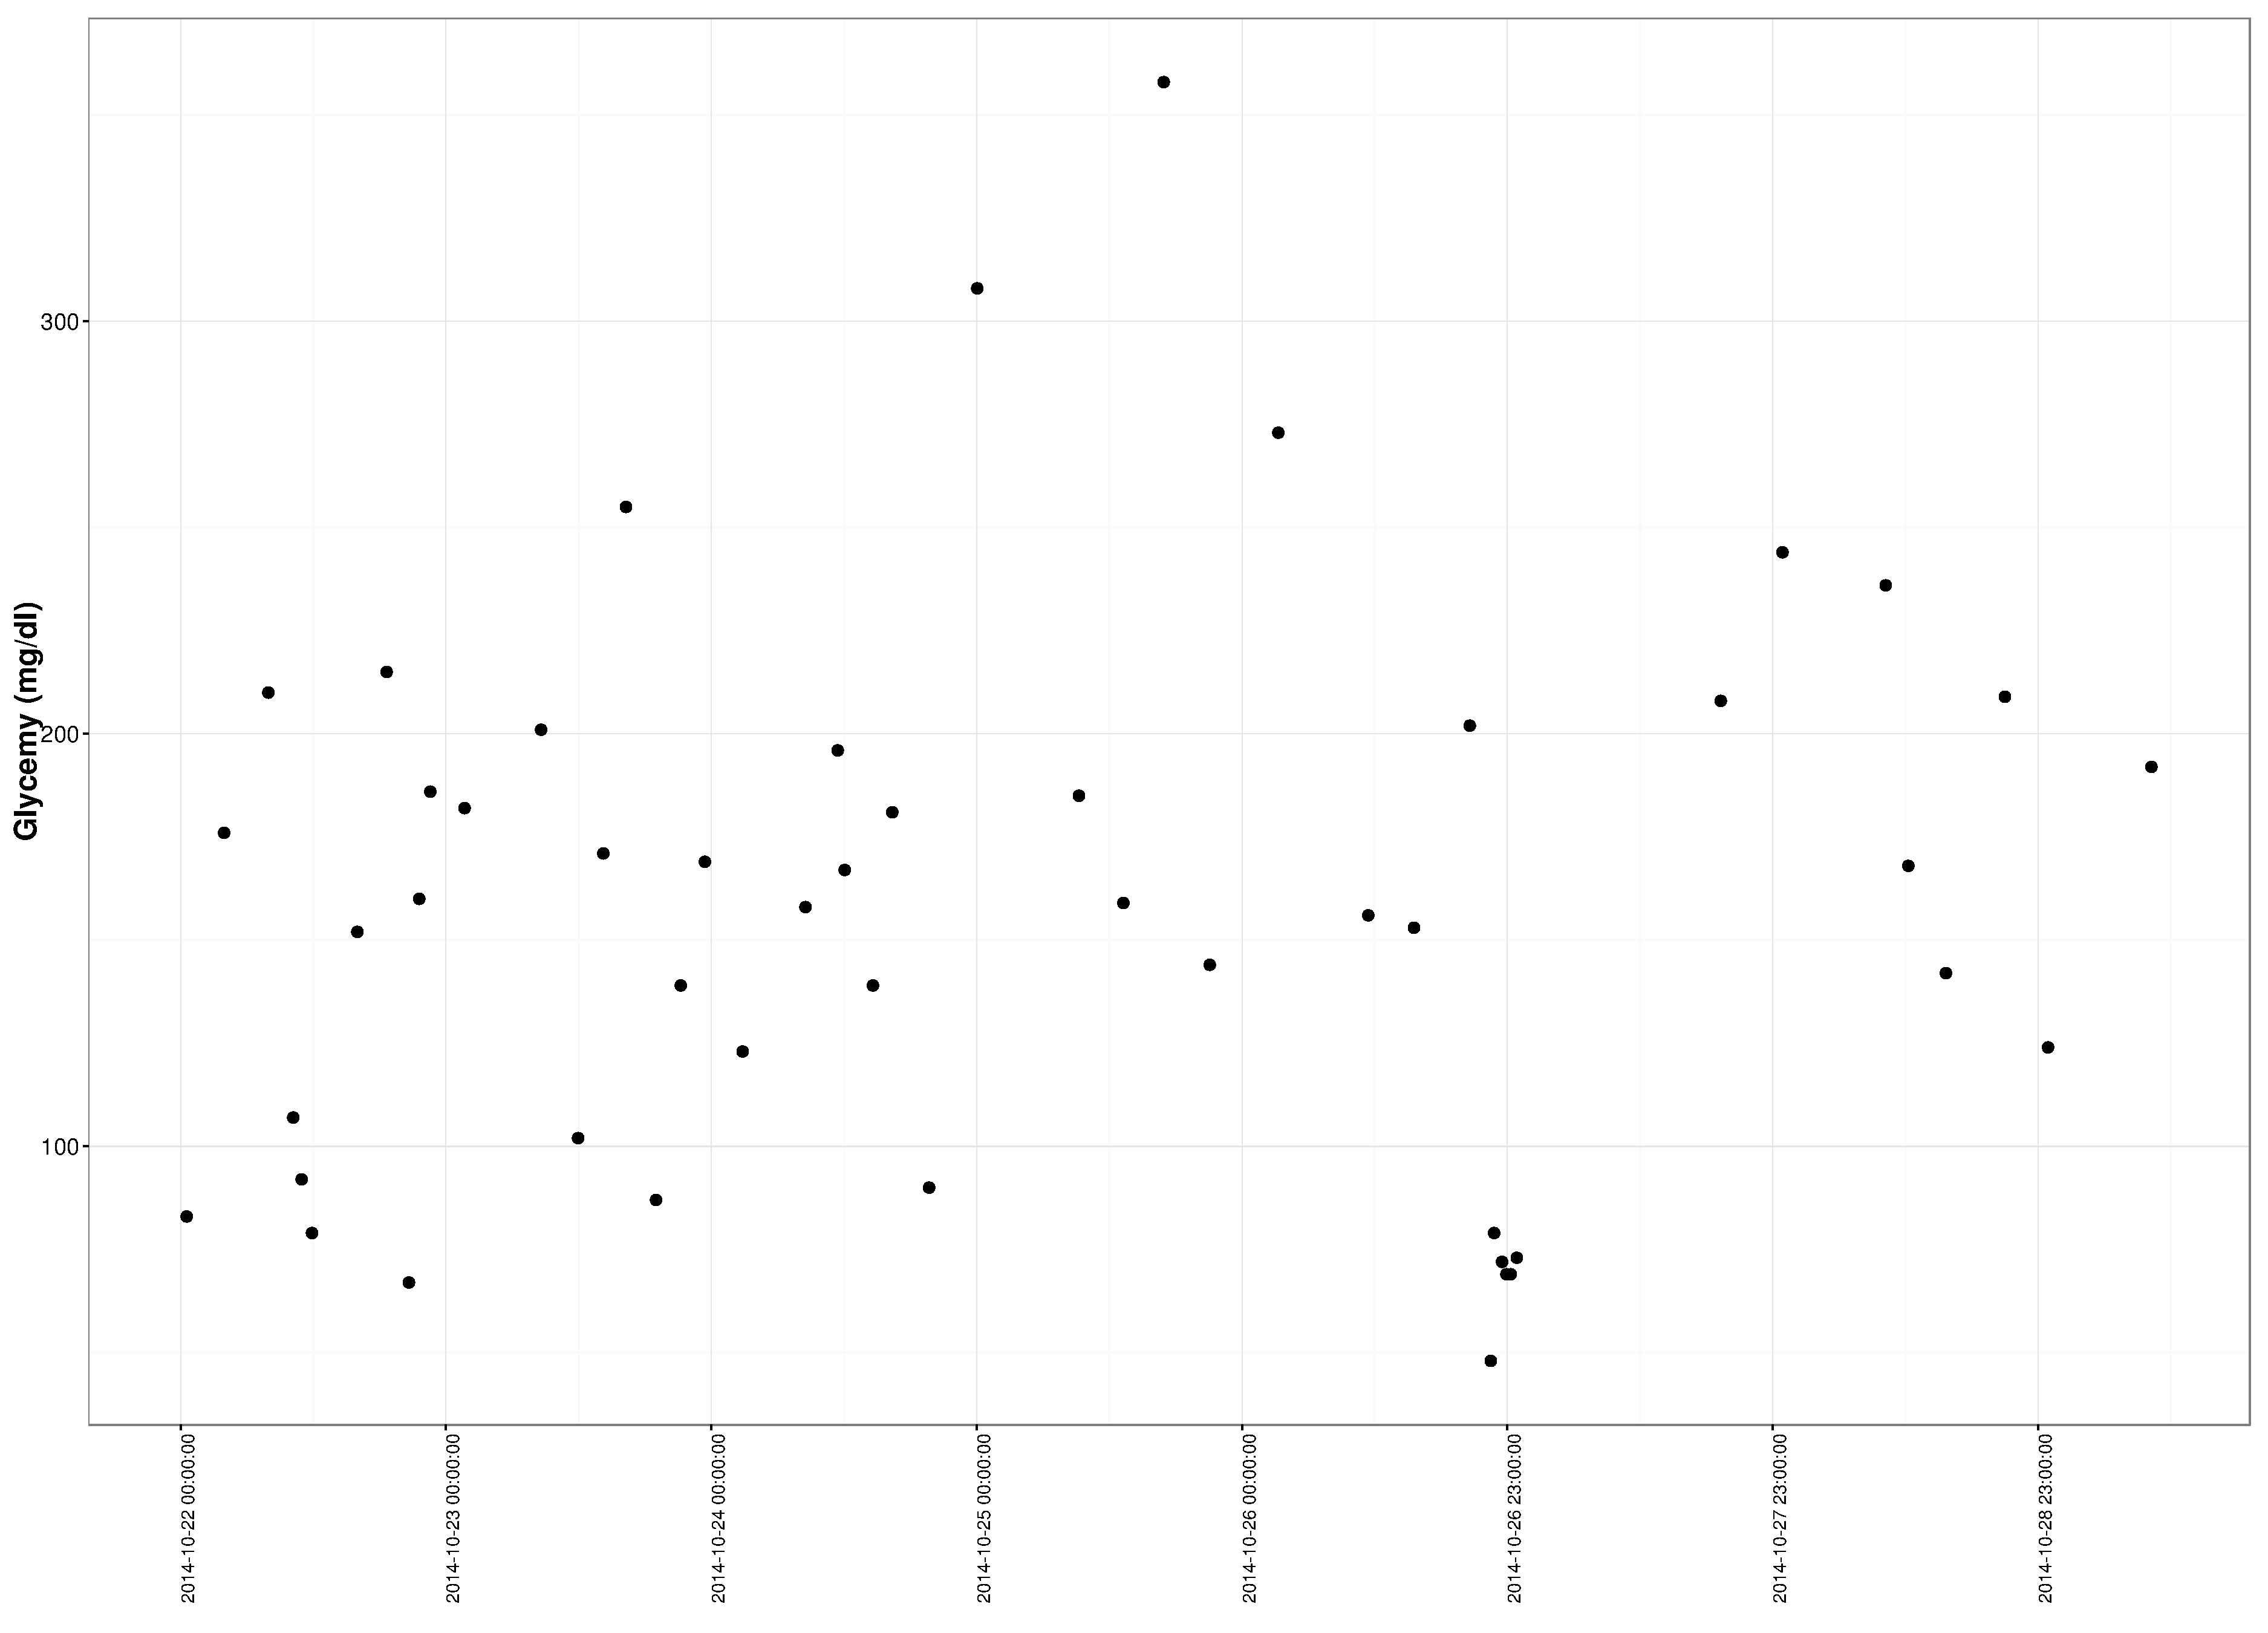
\includegraphics[height=\textwidth]{R/20141029.pdf}
\end{landscape}

\end{document}
